\documentclass[a4paper,12pt]{scrartcl}
\usepackage[utf8]{inputenc}
\usepackage[T1]{fontenc}
\usepackage[ngerman]{babel}
\usepackage{listings,lstautogobble}
\usepackage{xcolor}
\usepackage{scrpage2}
\usepackage{graphicx}

\renewcommand{\lstlistingname}{Quellcode}
\pagestyle{scrheadings}
\clearscrheadings
\clearscrplain
\clearscrheadfoot
\ihead[Julius Lehmann]{Julius Lehmann}
\ohead[\today]{\today}
\chead[\pagemark]{\pagemark}
\definecolor{RoyalBlue}{cmyk}{1, 0.50, 0, 0}

\lstset{
keywordstyle=\color{RoyalBlue},
breaklines=true,
breakautoindent=true,
numbers=left,
numberstyle=\tiny,
stepnumber=2,
numbersep=5pt,
keepspaces=false,
autogobble=true,
showstringspaces=false,
tabsize=2,
language=Java
}

%opening
\title{Dokumentation Aufgabe 2 - Ameisenfutter}
\author{Julius Lehmann}

\begin{document}
\maketitle
\section*{Lösungsidee:}
Das Programm sieht einen Simulationsschritt als Schleife über alle vorhandenen Ameisen an. Das heißt jede Ameise bekommt in einem Simulationsschritt eine neue Position zugewiesen. Die neue Position wird an Hand der Kriterien, die in der Aufgabenstellung formuliert sind, bestimmt, wobei bei dem Fall der zufälligen Bestimmung eines neuen Feldes eine weitere Bedingung hinzugefügt wurde. Da mir aufgefallen ist, dass die Ameisen oft wieder genau das Feld besuchen von dem sie im vorherigen Simulationsschritt gekommen sind, habe ich festgelegt, dass sie nur drei Felder zur Auswahl haben (ohne das bereits besuchte). Beim Start ist diese Bedingung außer Kraft gesetzt, da sie ja kein bereits besuchtes Feld besitzen.
Außerdem ist es möglich, dass sich mehrere Ameisen gleichzeitig auf einem Feld befinden und unabhängig voneinander einen Weg finden können. So ist ein schnellerer Programmablauf gewährleistet und die Logik ist einfacherer.

\section*{Umsetzung:}
Der Quellcode ist in der Sprache Java verfasst und die benutzte Grafik-Bibliothek ist JavaFX.
Um die Darstellung ansprechender zu gestalten, habe ich zum Darstellen der Objekte (Ameisen, Futter, \dots) kleine 18*18 Pixel Grafiken erstellt. Diese werden während der Simulation auf dem Spielfeld verschoben.
Das Programm ist in mehrere Dateien aufgeteilt:
\begin{description}
 \item[DrawArea] stellt die Zeichenfläche an sich und den Informationsaustausch zwischen der Simulation und dem Anwender dar.
 \item[Launcher] startet das Programm und reagiert auf Benutzerinteraktionen (Einstellungen, Start, Stopp)
 \item[Simulator] simuliert die Suche der Ameisen. Die Klasse stellt den Kern der Aufgabe dar und führt die Anforderungen der Simulation aus. Alle Werte werden hier verändert.
 \item[SimulationService] verwaltet die Simulation und führt die Berechnungen in einem neuen Thread aus. So reagiert die Grafik immer noch auf Interaktionen des Benutzers und die Simulation läuft trotzdem zügig im Hintergrund ab. Um einen reibungslosen Ablauf zu gewährleisten benutze ich die extra dafür vorgesehene API von JavaFX.
 \item[Speicher] speichert die Informationen der Simulation. Während Simulator diese verändert, greifen alle anderen nur auf die Informationen zu und verarbeiten diese.
 \item[Change] Objekt zur Beschreibung einer Veränderung der Simulation. Er hat die Koordinaten der Veränderungen und einen Buchstaben (P -- Pheromon, A -- Ameise, F -- Futter). Diese Veränderungen werden später sortiert weiterverarbeitet. Außerdem sind hashCode() und equals(Object) überschrieben, um doppelte Veränderungen zu vermeiden.
 \item[GChange] Objekt zur Beschreibung einer grafischen Veränderung. Es besteht aus dem grafischen Objekt und einem Wahrheitswert, der entweder besagt, dass dieses Objekt von der Spielfeldfläche verschwinden soll, oder es hinzugefügt werden soll.
 \item[XYPoint] Objekt zur Darstellung von Koordinaten im zweidimensionalen Raum. hashCode und equals überschrieben, um gleiche Punkte auseinander halten zu können.
\end{description}
Die letzten drei Objekte dienen lediglich der internen Verwaltung von Daten. Change und XYPoint überschreiben beide jeweils die hashCode- und equals-Funktion, sodass in einem HashSet (von mir oft verwendet) kein Objekt zweimal auftaucht. Das erleichtert später die Durchführung von Änderungen, da dann nicht mehr auf Duplikate getestet werden muss.
Die grafische Darstellung und die eigentliche Simulation sind voneinander getrennt. Die Simulation findet in einem neuen Thread statt und übergibt nach erfolgreichem Beenden die Daten an den Grafik-Thread, der diese dann darstellt. 

\subsection*{Simulation}
\subsubsection*{Simulator}
In Simulator ist die eigentliche Logik der Futtersuche verbaut:
\begin{lstlisting}[caption={Quelltext der Hauptsimulation in Simulator.java},label=sim]
 public Set<Change> simulate(int iterations, int phTimeout) {
    changes = new HashSet<Change>();
    /*
     * Entferne alte Pheromonspuren, immer wenn phTimeout-Schritte vorueber sind
     */
    for (int count = 0; count < iterations; count++) {
      speicher.steps++;
      if ((speicher.steps % phTimeout) == 0)
        for (Iterator<XYPoint> it = speicher.phero.iterator(); it.hasNext();) {
          XYPoint p = it.next();
          if (speicher.pheromone[p.x][p.y] == 0)
            it.remove();
          if (speicher.pheromone[p.x][p.y] > 0) {
            speicher.pheromone[p.x][p.y]--;
            changes.add(new Change('P', p.x, p.y));
          }
        }
      for (int aN = 0; aN < speicher.ameisen; aN++) // Durchlaufe alle Ameisen
      {
        Ameise cA = amArray[aN];
        if (cA.futter) // Futter im Inventar der Ameise?
        {
          // Falls Ameise im Nest, lege Futter ab und fuege dem Nest Futter hinzu
          if (cA.x == speicher.nestX && cA.y == speicher.nestY) {
            cA.futter = false;
            speicher.futterNest++;
          } else
          // ansonsten erhoehe aktuelle Pheromonkonzentration und begib dich auf das naechste Feld
          // in Richtung Nest
          {
            speicher.pheromone[cA.x][cA.y]++;
            speicher.phero.add(new XYPoint(cA.x, cA.y));
            changes.add(new Change('P', cA.x, cA.y));
            toNest(cA); // setze naechstes Feld in Richtung Nest
          }
        } else {
          // Falls kein Futter im Inventar
          if (speicher.futterVerteilung[cA.x][cA.y] > 0) {
            cA.futter = true; // nimm Futter auf
            speicher.futterVerteilung[cA.x][cA.y]--;
            Change aen = new Change('F', cA.x, cA.y);
            changes.add(aen);
          } else {
            if (nextPPos(cA))
              /*
               * Falls kein Futter im Inventar und keine Futterstelle gefunden, suche nach hoechster
               * Konzentration in Umgebung und setze Ameise gegebenenfalls dorthin. Ansonsten weiter
               * zu zufaelliger Positionierung
               */
              continue;
            else {
              List<int[]> availDirections = getAvailableDirections(cA);
              int rD = ThreadLocalRandom.current().nextInt(0, availDirections.size());
              setAPos(cA, availDirections.get(rD)[0], availDirections.get(rD)[1]);
              cA.lastDir = availDirections.get(rD)[2];
            }
          }
        }
      }
    }
    return changes;
  }
\end{lstlisting}
Am Anfang jeder Simulation wird ein neues HashSet für Veränderungen aufgebaut. Da die entsprechende Klasse zur Darstellung dieser Veränderungen (Change) die Funktionen equals und hashCode überschreibt, kann dieselbe Änderung mehrmals hinzugefügt werden, ohne dass sie später Einfuss auf die Berechnungen hat, da sie den gleichen hashCode besitzen und somit beim Iterieren nur einmal aufgerufen werden. Danach wird für eine gegebene Anzahl Simulationsschritte (Simulation wird n-mal wiederholt bis die Ergebnisse auf der Bildfläche erscheinen $\rightarrow$ das sorgt für eine bessere Performance und eine schnellere Analyse der Ergebnisse) die Simulation wiederholt.

Zuerst werden die Pheromonspuren aktualisiert und je nach eingestelltem Timeout um einen Schritt verringert. Eine lineare Abnahme ist zwar nicht ideal, da nach Erschöpfung der Futterquelle die Ameisenstraße noch einige Zeit \glqq{}sinnlos\grqq{} bestehen. Da aus der Aufgabenstellung heraus jedoch nicht deutlich gemacht wurde, welche Anforderungen die Verdunstungszeit erfüllen muss, habe ich es dabeui belassen.

Danach werden in einem Simulationsschritt alle Ameisen durchlaufen und je nach \glqq{}Umgebungsfaktoren\grqq{} die neuen Positionen bestimmt. Falls eine Ameise Futter in ihrem Inventar hat, wird sie auf dem schnellsten Weg zum Nest geschickt. Dabei wird die Differenz der aktuellen Position zur Nestposition ausgerechnet und die größere Komponente (x-, oder y-Achse) für das nächste Feld ausgewählt. (Bsp. Ameise a befindet sich auf Position (10|13). Das Nest ist bei (0|0). Das nächste Feld ist also (10|12), da der relative y-Wert (13) größer als der relative x-Wert (10) ist.)
Dann wird geprüft, ob die Ameise einen Futterplatz erreicht hat (d.h. an der Stelle (x|y) ist eine Portion an Futter > 0 vorhanden). Wenn ja, wird ihr eine Futterportion (bool'scher Wert) zugewiesen und dementsprechend Futter vom Futterplatz entfernt.
Schließlich wird die Basis-Routine aufgerufen. Die Ameise bekommt aus einer Liste von möglichen Positionen (innerhalb des Spielfeldes und nicht das vorherige Feld) eine zufällige zugewiesen.

\subsubsection*{SimulationService}
\begin{lstlisting}[caption={Grafikverwaltung in SimulationService}]
  /*
   * Verwaltet die Grafiken fuer die Objekte(Ameisen). Da die Ameisenobjekte wiederverwendet werden,
   * wird zusaetzlich zu einem Array von n (Ameisenanzahl) Grafiken noch eine Queue verwaltet, die
   * unbenutzte Indices zurueckgibt; ameisenPos ist eine Menge von allen auf der Simulationsflaeche
   * vorhandenen Grafiken. Soll eine Grafik entfernt werden, wird sie aus dieser Menge entfernt und
   * auch von der Flaeche. Falls die Grafik bestehen bleibt wird null zurueckgegeben
   */
  private GChange getAntChange(int x, int y, boolean draw) {
    XYPoint xy = new XYPoint(x, y);
    if (ameisenPos.containsKey(xy)) { // auf der Simulationsflaeche?
      if (!draw) {
        int index = ameisenPos.get(xy);
        ameisenPos.remove(xy);
        unusedViews.add(index);
        return new GChange(views[index], draw);
      } else
        return null;
    } else {
      if (!draw)
        return null;
      int index = unusedViews.poll();
      ameisenPos.put(xy, index);
      ImageView v = views[index];
      v.relocate(x * (width - 1) + 1, y * (width - 1) + 1);
      return new GChange(v, draw);
    }
  }
\end{lstlisting}
Jeder Simulationsaufruf bekommt einen eigenen Thread. In jedem Thread wird die Methode simulate(\dots{}) aus Simulator einmal aufgerufen, wobei iterations die Anzahl der Simulationsschritte bestimmt, d.h. es kann im Endeffekt länger als eine einzelne Simulation dauern. Nachdem dieser Thread (Task) abgeschlossen ist, wird das Event zurück an SimulationService gegeben, um dort zu prüfen, ob die Simulation gestoppt wurde. Falls ja, wird der Selbstaufruf von SimulationsService (ScheduledService) unterbrochen und keine Grafikupdates werden generiert. Das sichert eine problemlose Simulation, während bei einem unkontrollierten Abbruch nur Simulations-Teile behandelt worden wären, sodass das Ergebnis nicht gültig wäre.
Ist ein Task fertig mit der Arbeit, wird aus den gesammelten Change[s] alles nötige herausgefiltert und in GChange[s] umgewandelt. Wobei die Grafiken zum Darstellen der Ameisen wiederverwendet werden, da sich ihre Anzahl nicht im Laufe der gesamten Simulation ändert. Um später nicht eine bestimmte Grafik neu hinzuzufügen, die aber noch nicht entfernt wurde, werden die Updates nach Entfernen/Hinzufügen sortiert. Dieses Grafikupdate wird daraufhin an Launcher zurückgegeben, der dann nur noch die Objekte in DrawArea hinzufügt oder entfernt, wobei durch die vorherige Sortierung gewährleistet ist, dass erst die entsprechenden Objekte entfernt werden und erst dann neue hinzugefügt werden.

\subsection*{Grafik}
Die Grafik des Programmes besteht aus zwei FXML-Dateien und den Klassen DrawArea und Launcher.
Eine FXML-Datei beschreibt den Aufbau des Hauptfensters, das aus der Menüleiste und der Simulationsfläche besteht. Zum Starten der Simulation muss der Button "`Start"' im Simulation betätigt werden. Um die Simulation zu pausieren, bzw. die Einstellungen zu ändern, habe ich außerdem noch zwei weitere Schaltflächen hinzugefügt.

Über die Schaltfläche "`Einstellungen"' gelangt man schließlich zu einem neuen Fenster (die zweite FXML-Datei). Hier können viele Einstellungen, die für den Simulationsablauf entscheidend sind verändert werden. Unter anderem die Ameisenanzahl, Feldgröße und vor allem der Faktor für den Zeitraffer. Man muss dabei nicht alle Einstellungen verändern, da leere Felder mit den vorherigen Werten belegt werden.

Der Aufbau des Spielfeldes erfolgt durch Erzeugung einer maximal 1024*1024 Pixel großen Grafik, die den Hintergrund des Spielfeldes darstellt. Über "`BackgroundImage"' wird nun ein entsprechender Hintergrund für das Simulationsfeld gesetzt, das dann solange wiederholt wird, bis das Objekt komplett bedeckt ist. Mit Hilfe dieses Features wird die Grafik schnell und effizient aufgebaut, während die Nutzung von einzelnen Objekten deutliche Performance-Einbuße verursacht.

Die aktuellen Werte werden im Titel eines "`TitledPane"' dargestellt. Dadurch behält der Nutzer die Übersicht über die Anzahl der Ameisen auf einem Feld und Pheromonstärke, etc.

Damit die Grafik nicht während der Simulation hängt, habe ich eine Zeitspanne von 0,5 Sekunden zwischen zwei Grafikupdates eingefügt. Das sorgt für ein besseres Verständnis und eine bessere Beobachtung des Vorgangs.

\section*{Auffälligkeiten bei bestimmten Werten (Beispiele)}
Bei Änderung der
\begin{description}
\item[Ameisenanzahl] wird nicht nur die Simulationsflaeche voller, sondern auch die Geschwindigkeit des Futtersuchens wird schneller. Denn je mehr Ameisen auf dem Feld sind, desto größer ist die Wahrscheinlichkeit, dass sie in einer gegebenen Zeitspanne auf eine Futterquelle stoßen. Verringert man die Anzahl, geschieht das Umgekehrte.
\item[Nestposition] verändert sich der Weg zu den Rändern des Feldes und auch zu den Futterquellen. Das heißt, dass die Ameisen, um an das andere, entferntere Ende des Feldes zu gelangen, länger benötigen, als wenn das Nest in der Mitte liegt.
\item[Anzahl an Futterquellen] bekommen die Ameisen nicht nur weniger/mehr Futter, sondern es dauert im Schnitt auch länger/kürzer, bis sie eine Futterquelle gefunden haben, da die Wahrscheinlichkeit eine Quelle zu finden abnimmt/zunimmt.
\item[Verdunstungszeit] kann es entweder passieren, dass die Ameisen den Weg zur Futterquelle nicht wieder finden, da die Zeit zu kurz ist, oder dass sie auch noch lange Zeit nachdem die Quelle erschöpft ist auf der Spur bleiben (bei zu hoher Verdunstungszeit).
\end{description}
\begin{figure}[htbp]
\centering
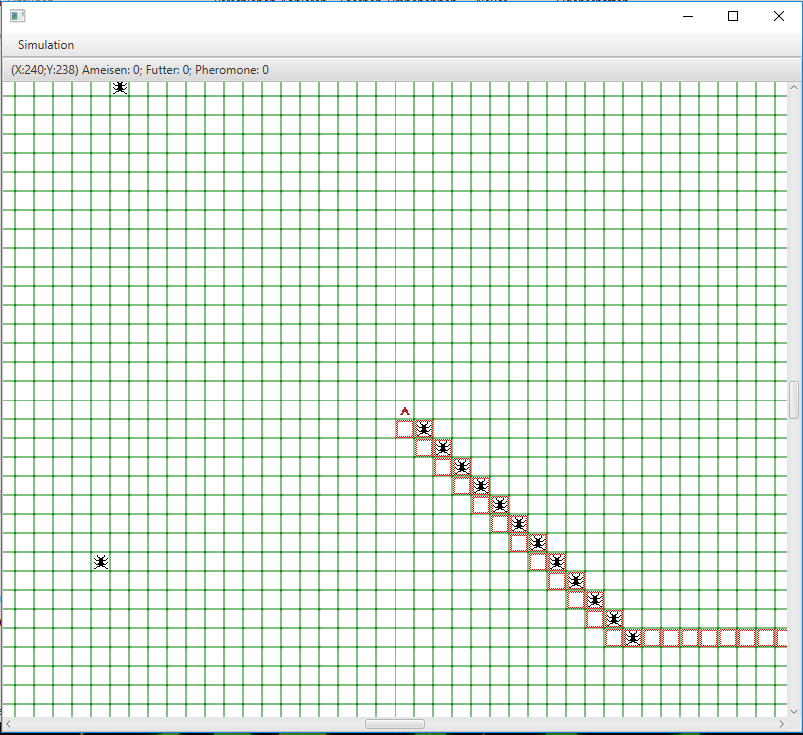
\includegraphics[scale=0.6]{Screenshot}
\caption{Screenshot de Simulation}
\end{figure}

\end{document}
